% Provenance (never printed): old seconde/premiere S material on the
% atmosphere (water vapour, saturation, cloud formation, the vertical motion
% of air) and enseignement scientifique premiere (water cycle); see
% sources/book2/PROVENANCE.md. Every saturation value, lapse rate,
% condensation level and the lee-wind example are computed in
% figdata/grade-10/clouds.py from the IAPWS saturation curves; the soundings
% are invented examples, said so in the text.
\chapter{Waarom wolken ontstaan}\label{ch:g10:why-clouds-form}

Op een zomers terras staat een glas ijswater op tafel. Binnen een minuut is de
buitenkant bedekt met piepkleine druppels, en aan de voet verspreidt zich een
kringetje water. Het water is niet door het glas gelekt: het kwam uit de lucht,
die werd afgekoeld waar ze het koude glas raakte. Een paar uur later gebeurt
kilometers boven de vlakte hetzelfde op grote schaal: bellen warme lucht
stijgen op, koelen af, en op een bepaalde hoogte verschijnt het water dat ze
meevoeren als de witte stapels met een platte onderkant die cumulus heten. Dit
hoofdstuk legt uit hoeveel waterdamp lucht kan bevatten, waarom stijgende lucht
afkoelt, op welke hoogte wolken ontstaan, waarom ze op sommige dagen plat
blijven en op andere uitgroeien tot onweerswolken, en hoe piepkleine
wolkendruppeltjes regen en sneeuw worden.

\begin{omfigure}
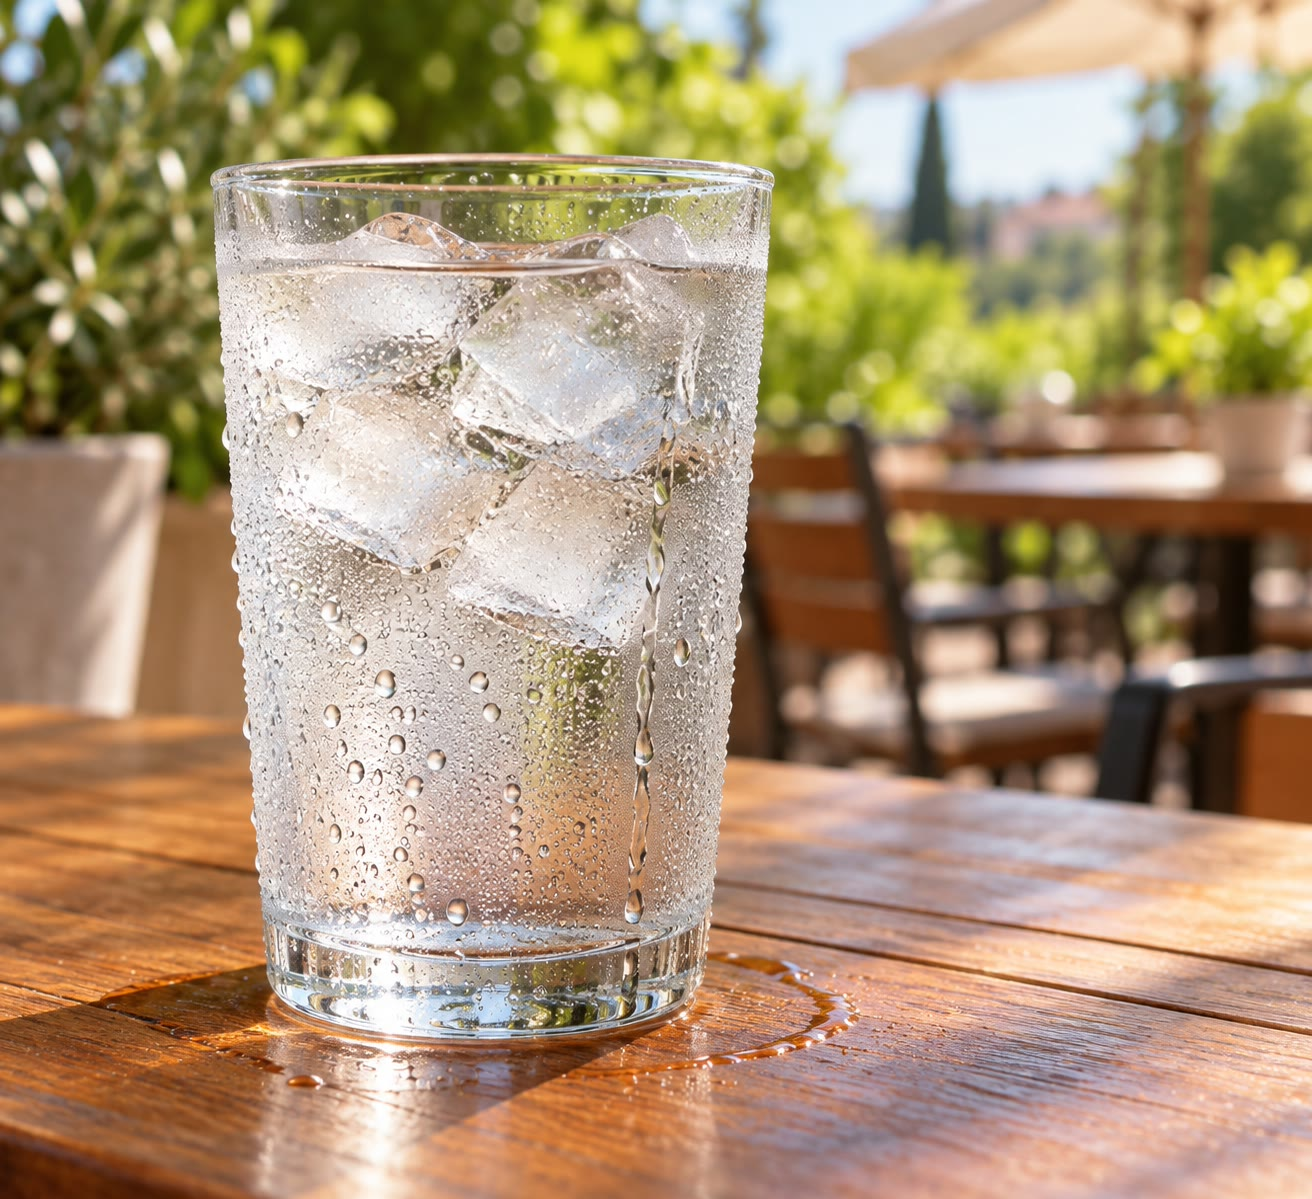
\includegraphics[width=0.5\linewidth]{images/book2/ai/g10-cold-glass.jpg}

{\small Een glas ijswater op een zomers terras: aan de buitenkant ontstaan
druppels, waar de lucht die het glas raakt wordt afgekoeld.}
\end{omfigure}

\begin{recall}
Wolken bestaan uit piepkleine waterdruppeltjes of ijskristallen; ze worden naar
hun vorm en hoogte in families ingedeeld, en ze geven regen, sneeuw en hagel,
die je met een regenmeter meet (Boek 1, jaar 4). De temperatuur van de lucht
daalt met de hoogte in de onderste laag van de atmosfeer, gemiddeld met
ongeveer \qty{6.5}{\degreeCelsius} per kilometer; dat is de verticale
temperatuurgradiënt, en fronten scheiden luchtmassa's met verschillende
temperaturen (Boek 1, jaar 8). De druk daalt met de hoogte (de
natuurkundeboeken). Water verdampt en condenseert, en verdamping neemt \omterm{def:g10:earth-energy-budget:latent-heat}{latente
warmte} op die condensatie teruggeeft (de natuurkundeboeken en
\cref{ch:g10:earth-energy-budget}).
\end{recall}
% ledger: nasa:grc-atmosphere

\section{Waterdamp en verzadiging}

Lucht bevat altijd wat waterdamp, een onzichtbaar gas. Hoeveel ze kan bevatten,
hangt vooral af van haar temperatuur.

\begin{definition}[Verzadiging; relatieve luchtvochtigheid]\label{def:g10:why-clouds-form:humidity}
Lucht is \emph{verzadigd}\index{verzadiging} wanneer ze de grootste massa
waterdamp bevat die ze bij haar temperatuur kan vasthouden, haar
\emph{verzadigingsgehalte}; elke extra damp condenseert tot druppeltjes. De
\emph{relatieve luchtvochtigheid}\index{relatieve luchtvochtigheid} van lucht
is haar gehalte aan waterdamp gedeeld door haar verzadigingsgehalte bij dezelfde
temperatuur en druk, uitgedrukt als percentage.
\end{definition}

Het watergehalte van lucht wordt hier gemeten in gram damp per kilogram droge
lucht (\unit{g/kg}): een luchtpakketje dat stijgt of daalt zonder water te
winnen of te verliezen, houdt hetzelfde gehalte, ook al zet het uit.

\begin{omfigure}
\begin{tikzpicture}
\begin{axis}[omrecord, width=0.88\linewidth, height=6.2cm, xmin=-10, xmax=40,
  ymin=0, ymax=50, xlabel={temperatuur (\unit{\degreeCelsius})},
  ylabel={verzadigingsgehalte (\unit{g/kg})}, xtick={-10,0,...,40},
  tick label style={font=\small}, label style={font=\small}]
\addplot[omDef!85!black, thick] table[x=T_C, y=ws_gkg] {figdata/out/grade-10-clouds-sat.dat};
\addplot[only marks, mark=*, mark size=1.8pt, omThm!85!black] coordinates {(28,11.37)};
\addplot[only marks, mark=o, mark size=1.8pt, omThm!85!black] coordinates {(16,11.37)};
\draw[->, omThm!85!black, thick] (axis cs:27.2,11.37) -- (axis cs:16.9,11.37);
\node[anchor=north, font=\footnotesize, omThm!85!black] at (axis cs:28,10.6) {lucht van \qty{28}{\degreeCelsius}};
\node[anchor=south east, font=\footnotesize, omThm!85!black] at (axis cs:15.5,12.2) {dauwpunt};
\node[anchor=south east, font=\footnotesize, omDef!85!black, align=right] at (axis cs:31,34) {boven de kromme:\\damp condenseert};
\node[anchor=south west, font=\footnotesize, omDef!85!black] at (axis cs:31,2.5) {niet verzadigd};
\node[anchor=north west, font=\footnotesize, omDef!85!black] at (axis cs:34,31.5) {verzadiging};
\end{axis}
\end{tikzpicture}

{\small De grootste massa waterdamp die een kilogram lucht kan bevatten, tegen
de temperatuur, bij de druk op zeeniveau (boven vloeibaar water; berekend met de
internationale standaard voor water). Lucht van \qty{28}{\degreeCelsius} met
\qty{11.4}{g/kg} (stip) is ver van \omterm{def:g10:why-clouds-form:humidity}{verzadiging}; afgekoeld zonder water te
verliezen, raakt ze \omterm{def:g10:why-clouds-form:humidity}{verzadigd} bij \qty{16}{\degreeCelsius} (cirkel).}
\end{omfigure}
% ledger: iapws:vapour-pressure, ciaaw:abridged-2024, earth:Mmol, const:R (computed in figdata/grade-10/clouds.py)

De kromme stijgt steil: \qty{3.8}{g/kg} bij \qty{0}{\degreeCelsius},
\qty{14.7}{g/kg} bij \qty{20}{\degreeCelsius}, \qty{27.2}{g/kg} bij
\qty{30}{\degreeCelsius}. Elke \qty{10}{\degreeCelsius} opwarming verdubbelt
bijna het water dat de lucht kan bevatten. Daarom kan tropische lucht
stortregens meevoeren, en bevat de lucht van een poolwinter, zelfs \omterm{def:g10:why-clouds-form:humidity}{verzadigd},
bijna niets.

\begin{definition}[Dauwpunt]\label{def:g10:why-clouds-form:dew-point}
Het \emph{dauwpunt}\index{dauwpunt} van lucht is de temperatuur waartoe ze moet
worden afgekoeld, met behoud van haar watergehalte en haar druk, om \omterm{def:g10:why-clouds-form:humidity}{verzadigd} te
raken.
\end{definition}

\begin{method}[Relatieve luchtvochtigheid en dauwpunt uit een tabel]\label{met:g10:why-clouds-form:table}
\begin{enumerate}
  \item Lees in de tabel het verzadigingsgehalte bij de temperatuur van de lucht af.
  \item \omterm{def:g10:why-clouds-form:humidity}{Relatieve luchtvochtigheid}: deel het watergehalte van de lucht erdoor.
  \item \omterm{def:g10:why-clouds-form:dew-point}{Dauwpunt}: zoek in de tabel de temperatuur waarvan het
        verzadigingsgehalte gelijk is aan het watergehalte van de lucht.
\end{enumerate}
\end{method}

\begin{example}[Een zomerochtend]\label{ex:g10:why-clouds-form:morning}
% ledger: iapws:vapour-pressure (values computed in figdata/grade-10/clouds.py)
Bij \qty{20}{\degreeCelsius} bevat de lucht \qty{11.4}{g/kg}. Het
verzadigingsgehalte bij \qty{20}{\degreeCelsius} is \qty{14.7}{g/kg}, dus de
\omterm{def:g10:why-clouds-form:humidity}{relatieve luchtvochtigheid} is $11.4/14.7 \approx \qty{78}{\percent}$. Het
verzadigingsgehalte is \qty{11.4}{g/kg} bij \qty{16}{\degreeCelsius}: dat is
het \omterm{def:g10:why-clouds-form:dew-point}{dauwpunt}. 's Middags heeft dezelfde lucht, opgewarmd tot
\qty{28}{\degreeCelsius} (verzadigingsgehalte \qty{24.1}{g/kg}), een \omterm{def:g10:why-clouds-form:humidity}{relatieve
luchtvochtigheid} van maar \qty{47}{\percent} --- met precies hetzelfde water erin.
\end{example}

Het glas uit de opening is kouder dan het \omterm{def:g10:why-clouds-form:dew-point}{dauwpunt} van de lucht eromheen: de
lucht die het raakt, wordt onder haar \omterm{def:g10:why-clouds-form:dew-point}{dauwpunt} afgekoeld en geeft water af op
het glas. In een heldere nacht verliezen gras en autodaken warmte door
infrarood naar de hemel uit te stralen, en worden ze kouder dan de lucht: er
vormt zich dauw op, of rijp onder \qty{0}{\degreeCelsius}. Wanneer een hele
luchtlaag bij de grond tot haar \omterm{def:g10:why-clouds-form:dew-point}{dauwpunt} afkoelt, ontstaan er druppeltjes in de
lucht zelf: mist.

\begin{omfigure}
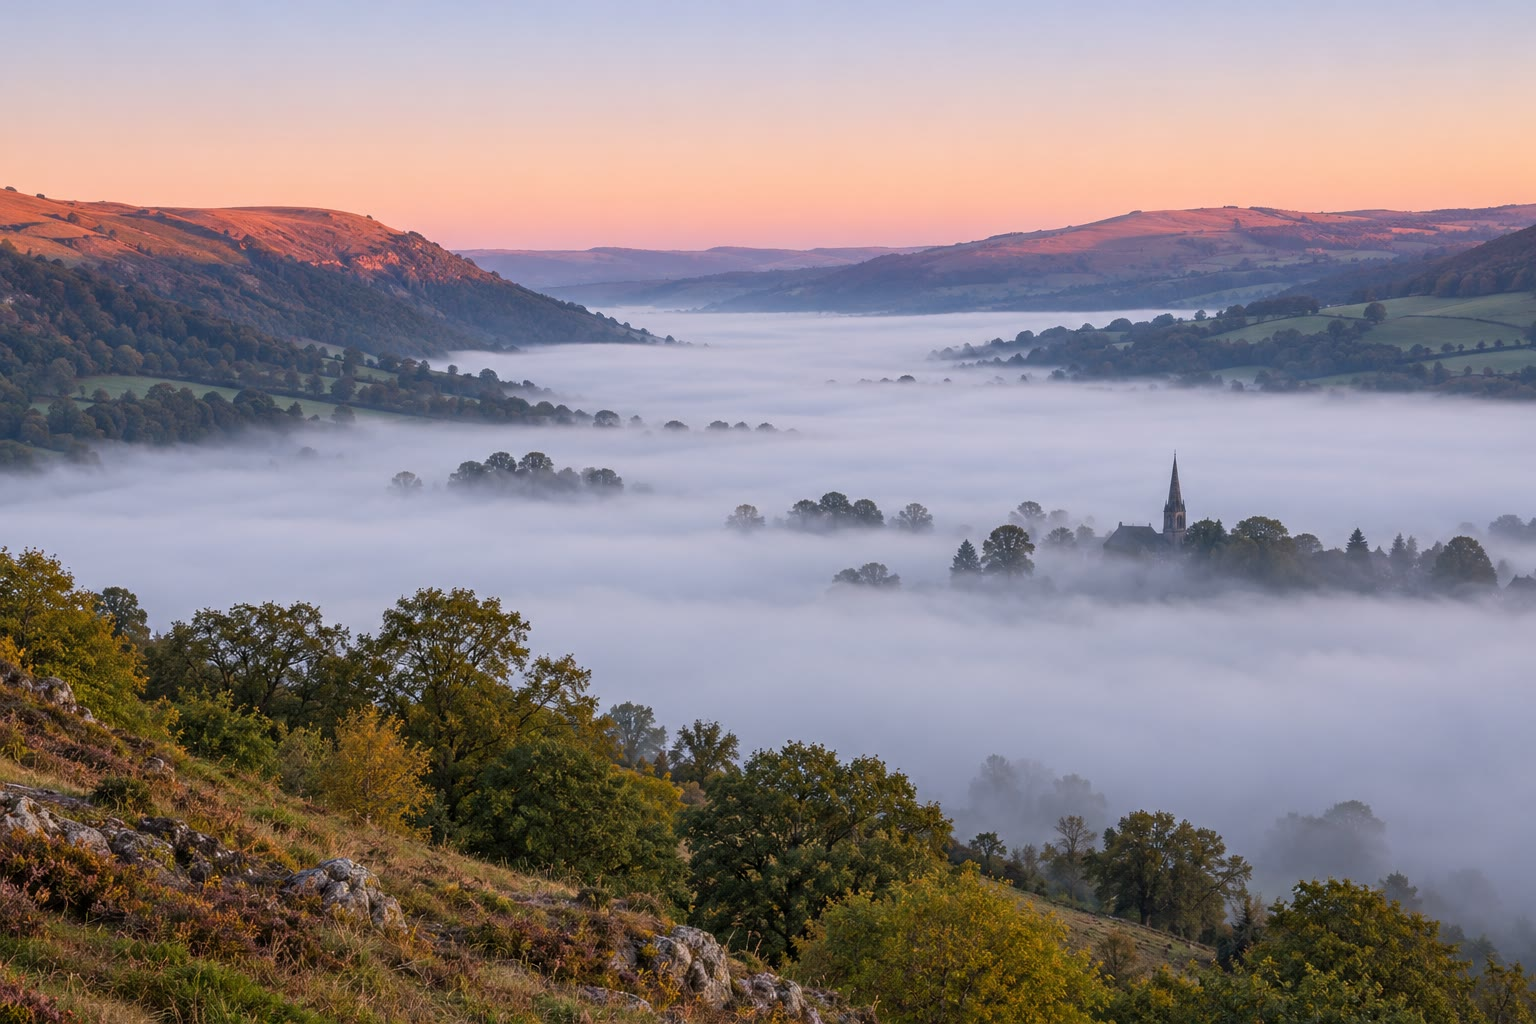
\includegraphics[width=0.75\linewidth]{images/book2/ai/g10-valley-fog.jpg}

{\small Mist die bij zonsopgang een dal vult. Tijdens de heldere nacht koelde
de grond af, de koude lucht stroomde het dal in, en daar koelde ze af tot onder
haar \omterm{def:g10:why-clouds-form:dew-point}{dauwpunt}.}
\end{omfigure}

\section{Stijgende lucht koelt af}

De meeste wolken ontstaan niet doordat lucht iets kouds raakt. Ze ontstaan
doordat lucht opstijgt. De druk daalt met de hoogte; een stijgend luchtpakketje
zet uit en duwt de omringende lucht weg, en de energie voor dat werk komt uit
het pakketje zelf.

\begin{definition}[Adiabatische afkoeling; droogadiabatische gradiënt]\label{def:g10:why-clouds-form:adiabatic}
\emph{Adiabatische afkoeling}\index{adiabatische afkoeling} is de afkoeling van
een luchtpakketje dat uitzet zonder warmte met zijn omgeving uit te wisselen.
De snelheid waarmee stijgende onverzadigde lucht zo afkoelt, is de
\emph{droogadiabatische gradiënt}\index{droogadiabatische gradient@droogadiabatische gradiënt}, ongeveer
\qty{9.8}{\degreeCelsius} per kilometer stijging; dalende lucht warmt in
hetzelfde tempo op.
\end{definition}

\begin{proposition}[De droogadiabatische gradiënt]\label{prop:g10:why-clouds-form:dry-rate}
De \omterm{def:g10:why-clouds-form:adiabatic}{droogadiabatische gradiënt} is $g/c_p$, met $g = \qty{9.81}{m/s^2}$ en $c_p
\approx \qty{1005}{J.kg^{-1}.K^{-1}}$ de energie die een kilogram lucht bij
constante druk één graad opwarmt: $9.81/1005 \approx
\qty{0.0098}{\degreeCelsius/m}$, dat is \qty{9.8}{\degreeCelsius/km}.
(Aangenomen: het bewijs hoort bij de natuurkundeboeken.)
\end{proposition}
% ledger: const:gn, const:R, earth:Mmol (c_p of dry air computed as (7/2)R/M in figdata/grade-10/clouds.py)

Ook het \omterm{def:g10:why-clouds-form:dew-point}{dauwpunt} van het pakketje daalt terwijl het stijgt, maar langzaam: het
watergehalte blijft gelijk, terwijl de lagere druk de damp iets makkelijker
verzadigt. De berekening voor lucht bij de grond geeft ongeveer
\qty{1.8}{\degreeCelsius} per kilometer. De temperatuur van het pakketje komt
dus voor elke kilometer die het klimt ongeveer $9.8 - 1.8 = \qty{8}{\degreeCelsius}$
dichter bij zijn \omterm{def:g10:why-clouds-form:dew-point}{dauwpunt}.
% ledger: iapws:vapour-pressure (dew-point rate computed in figdata/grade-10/clouds.py)

\begin{definition}[Condensatieniveau]\label{def:g10:why-clouds-form:condensation-level}
Het \emph{condensatieniveau}\index{condensatieniveau} van een luchtpakketje is
de hoogte waarop het bij het stijgen \omterm{def:g10:why-clouds-form:humidity}{verzadigd} raakt. Daarboven condenseert
water: het condensatieniveau is de platte onderkant van de wolken die de
stijgende lucht vormt.
\end{definition}

\begin{proposition}[Hoogte van het condensatieniveau]\label{prop:g10:why-clouds-form:lcl}
Lucht die van de grond opstijgt met temperatuur $T$ en \omterm{def:g10:why-clouds-form:dew-point}{dauwpunt} $T_d$
(in \unit{\degreeCelsius}), raakt \omterm{def:g10:why-clouds-form:humidity}{verzadigd} op ongeveer
\[
  z = \frac{T - T_d}{8}\ \text{km} = \qty{125}{m} \times (T - T_d).
\]
\end{proposition}

\begin{proof}
Op een hoogte $z$ (in km) is de temperatuur van het pakketje $T - 9.8\,z$ en zijn
\omterm{def:g10:why-clouds-form:dew-point}{dauwpunt} $T_d - 1.8\,z$. Het is \omterm{def:g10:why-clouds-form:humidity}{verzadigd} wanneer die gelijk zijn:
$T - 9.8\,z = T_d - 1.8\,z$, dus $8\,z = T - T_d$ en $z = (T - T_d)/8$ km.
Een achtste kilometer is \qty{125}{m}.
\end{proof}

\begin{example}[Een cumulus in de middag]\label{ex:g10:why-clouds-form:base}
% ledger: iapws:vapour-pressure (exact ascent computed in figdata/grade-10/clouds.py: 1.51 km)
In de middag van \cref{ex:g10:why-clouds-form:morning} is de lucht bij de grond
\qty{28}{\degreeCelsius}, met een \omterm{def:g10:why-clouds-form:dew-point}{dauwpunt} van \qty{16}{\degreeCelsius}.
Opstijgende bellen raken \omterm{def:g10:why-clouds-form:humidity}{verzadigd} op $125 \times 12 = \qty{1500}{m}$: de
cumuluswolken hebben hun platte onderkant op ongeveer \qty{1.5}{km} hoogte. 's
Ochtends, bij \qty{20}{\degreeCelsius}, zou dezelfde lucht al op maar
$125 \times 4 = \qty{500}{m}$ zijn gecondenseerd: de wolkenbasis stijgt in de
loop van de dag, terwijl de grond opwarmt.
\end{example}

\section{Stabiele en onstabiele lucht}

Of een stijgend pakketje blijft stijgen, hangt af van de lucht eromheen. Een
pakketje dat warmer is dan zijn omgeving, is lichter dan de lucht die het
verdringt en stijgt, zoals een heteluchtballon; een pakketje dat kouder is dan
zijn omgeving, zakt terug.

\begin{definition}[Stabiele lucht; onstabiele lucht]\label{def:g10:why-clouds-form:stability}
Lucht is \emph{stabiel}\index{stabiele lucht} wanneer een pakketje dat omhoog
wordt geduwd kouder wordt dan de lucht eromheen, en dus terugzakt naar waar het
begon. Ze is \emph{onstabiel}\index{onstabiele lucht} wanneer het pakketje warmer
wordt dan de lucht eromheen en uit zichzelf blijft stijgen.
\end{definition}

Het stijgende pakketje koelt af met de \omterm{def:g10:why-clouds-form:adiabatic}{droogadiabatische gradiënt},
\qty{9.8}{\degreeCelsius} per kilometer, zolang het niet \omterm{def:g10:why-clouds-form:humidity}{verzadigd} is. Zodra het
\omterm{def:g10:why-clouds-form:humidity}{verzadigd} is, koelt het langzamer af: condensatie geeft \omterm{def:g10:earth-energy-budget:latent-heat}{latente warmte} af aan het
pakketje. De berekening geeft ongeveer \qty{4.7}{\degreeCelsius} per kilometer in
warme lucht bij de grond, ongeveer \num{5.8} bij \qty{0}{\degreeCelsius}, en meer
in de koude lucht hogerop, waar weinig water overblijft om te condenseren; dat
is de natadiabatische gradiënt. (De formule ervan wordt afgeleid in de
universitaire boeken.)
% ledger: nist:water-latent, iapws:vapour-pressure (saturated rates computed in figdata/grade-10/clouds.py)

\begin{method}[Is deze lucht stabiel?]\label{met:g10:why-clouds-form:stable}
\begin{enumerate}
  \item Zoek hoe snel de temperatuur van de omringende lucht met de hoogte daalt
        (de verticale temperatuurgradiënt, uit een ballonpeiling).
  \item Vergelijk die met de snelheid waarmee het pakketje afkoelt: de droge
        gradiënt, ongeveer \qty{9.8}{\degreeCelsius/km}, onder zijn
        \omterm{def:g10:why-clouds-form:condensation-level}{condensatieniveau}; de natte gradiënt, ongeveer
        \qty{5}{\degreeCelsius/km}, erboven.
  \item Koelt de omgeving langzamer af dan het pakketje, dan wordt het pakketje
        kouder: \omterm{def:g10:why-clouds-form:stability}{stabiel}. Koelt ze sneller af, dan wordt het pakketje warmer:
        \omterm{def:g10:why-clouds-form:stability}{onstabiel}. Een laag waarin de temperatuur met de hoogte \emph{stijgt},
        is zeer \omterm{def:g10:why-clouds-form:stability}{stabiel}: ze houdt stijgende lucht tegen als een deksel.
\end{enumerate}
\end{method}

Met de gemiddelde gradiënt van ongeveer \qty{6.5}{\degreeCelsius/km} is lucht
\omterm{def:g10:why-clouds-form:stability}{stabiel} zolang ze onverzadigd is (het pakketje koelt sneller af) en \omterm{def:g10:why-clouds-form:stability}{onstabiel}
zodra ze \omterm{def:g10:why-clouds-form:humidity}{verzadigd} is (het pakketje koelt langzamer af). Zulke lucht heet
voorwaardelijk \omterm{def:g10:why-clouds-form:stability}{onstabiel}: ze is \omterm{def:g10:why-clouds-form:stability}{stabiel} tenzij iets haar tot haar
\omterm{def:g10:why-clouds-form:condensation-level}{condensatieniveau} optilt, en dan groeit de wolk uit zichzelf.

\begin{omfigure}
\begin{tikzpicture}
\begin{axis}[omrecord, width=0.9\linewidth, height=7.6cm, xmin=-30, xmax=36,
  ymin=0, ymax=6, xlabel={temperatuur (\unit{\degreeCelsius})}, ylabel={hoogte (km)},
  xtick={-30,-20,...,30}, ytick={0,1,...,6},
  legend style={at={(0.02,0.98)}, anchor=north west, font=\footnotesize, draw=black!30, fill=white},
  tick label style={font=\small}, label style={font=\small}]
\fill[omDef!10] (axis cs:-30,1.51) rectangle (axis cs:36,3.96);
\addplot[black!60, thick] table[x=T_C, y=z_km] {figdata/out/grade-10-clouds-envA.dat};
\addlegendentry{peiling A}
\addplot[omProp!90!black, thick, densely dotted] table[x=T_C, y=z_km] {figdata/out/grade-10-clouds-envB.dat};
\addlegendentry{peiling B}
\addplot[omThm!85!black, very thick] table[x=T_C, y=z_km] {figdata/out/grade-10-clouds-parcel.dat};
\addlegendentry{stijgend pakketje}
\addplot[omMeth!85!black, thick, dashed] table[x=Td_C, y=z_km] {figdata/out/grade-10-clouds-dew.dat};
\addlegendentry{zijn dauwpunt}
\draw[black!50, dashed] (axis cs:-30,1.51) -- (axis cs:36,1.51);
\node[anchor=south west, font=\footnotesize] at (axis cs:-29.5,1.53) {condensatieniveau};
\node[anchor=north east, font=\footnotesize, omDef!80!black] at (axis cs:35.5,3.9) {wolk bij A};
\end{axis}
\end{tikzpicture}

{\small Een pakketje dat van de grond opstijgt bij \qty{28}{\degreeCelsius} met
een \omterm{def:g10:why-clouds-form:dew-point}{dauwpunt} van \qty{16}{\degreeCelsius} (berekend): het koelt af met de droge
gradiënt tot zijn temperatuur op \qty{1.5}{km} zijn \omterm{def:g10:why-clouds-form:dew-point}{dauwpunt} bereikt, en daarna
met de tragere natte gradiënt. Twee verzonnen peilingen: in A is het pakketje
warmer dan zijn omgeving van \qty{1.5}{km} tot aan de warme laag bij
\qty{4}{km}, en daartussen groeit een cumulus (gearceerd); in B houdt warmere
lucht boven de grond het pakketje overal kouder dan zijn omgeving: \omterm{def:g10:why-clouds-form:stability}{stabiele
lucht}, geen cumulus.}
\end{omfigure}
% ledger: iapws:vapour-pressure, nist:water-latent (parcel computed in figdata/grade-10/clouds.py; soundings invented)

Wanneer de lucht \omterm{def:g10:why-clouds-form:stability}{stabiel} is en toch wordt opgetild --- over een berg, of langs
een front --- spreiden de wolken die ontstaan zich uit in vlakke grijze lagen:
stratus. Wanneer ze \omterm{def:g10:why-clouds-form:stability}{onstabiel} is, bollen de wolken in stapels op: cumulus, en,
als de instabiliteit hoog genoeg reikt, de cumulonimbus van onweersbuien, waarvan
de top zich uitspreidt tot een aambeeld waar hij de zeer \omterm{def:g10:why-clouds-form:stability}{stabiele lucht} boven de
onderste laag van de atmosfeer ontmoet.

\begin{omfigure}
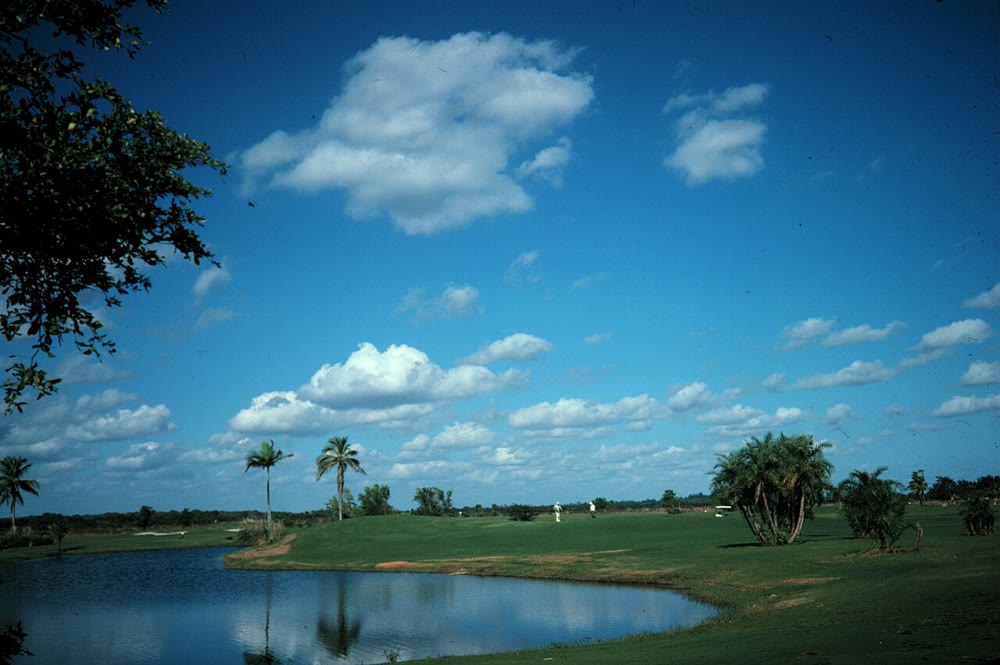
\includegraphics[height=4.5cm]{images/book2/g10-noaa-fair-weather-cumulus.jpg}\hspace{0.6em}%
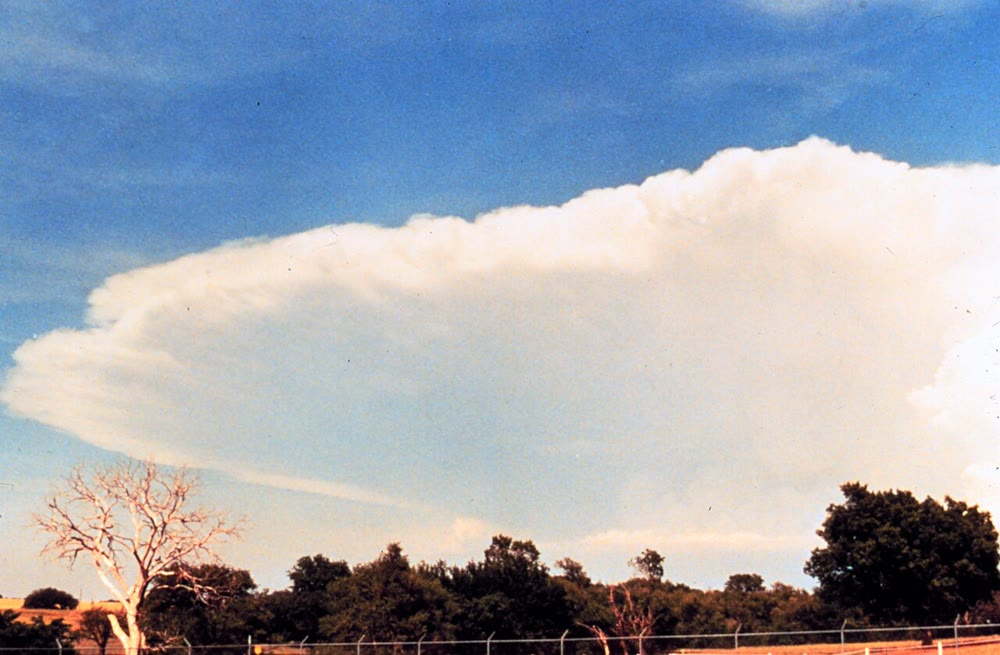
\includegraphics[height=4.5cm]{images/book2/g10-noaa-cumulonimbus-anvil.jpg}

{\small Links: mooiweercumulus boven Florida, met een platte onderkant op hun
\omterm{def:g10:why-clouds-form:condensation-level}{condensatieniveau}. Foto: Ralph F. Kresge, NOAA (publiek domein). Rechts: het
aambeeld van een cumulonimbus in de beginfase van een onweer. Foto: NOAA
National Severe Storms Laboratory (publiek domein).}
\end{omfigure}

\section{Vier manieren om lucht op te tillen}

Lucht stijgt om vier redenen.
\begin{itemize}
  \item \textbf{Verwarming van onderen.} Op een zonnige dag verwarmt de grond de
        lucht erboven; van de warmste plekken stijgen bellen warme lucht op. Zij
        geven de cumuluswolken van de middag.
  \item \textbf{Bergen.} Wind die tegen een bergketen waait, wordt langs de
        helling omhoog gedwongen.
  \item \textbf{Fronten.} Waar warme en koude luchtmassa's elkaar ontmoeten,
        stijgt de lichtere warme lucht boven de koude lucht uit, of schuift de
        koude lucht eronder (Boek 1, jaar 8).
  \item \textbf{Convergentie.} Wanneer winden bij de grond samenstromen, kan de
        lucht nergens anders heen dan omhoog, zoals in de gordel van stijgende
        lucht bij de evenaar en in het centrum van een depressie.
\end{itemize}

\begin{method}[Een pakketje over een berg volgen]\label{met:g10:why-clouds-form:mountain}
\begin{enumerate}
  \item Zoek het \omterm{def:g10:why-clouds-form:condensation-level}{condensatieniveau} met de regel van 125 meter; tot daar koelt
        het pakketje af met \qty{9.8}{\degreeCelsius/km}.
  \item Vandaar tot de top koelt het af met de natte gradiënt; het water dat
        condenseert, valt als regen of sneeuw aan de loefzijde.
  \item Voorbij de top daalt het pakketje, onverzadigd: het warmt helemaal naar
        beneden op met \qty{9.8}{\degreeCelsius/km}.
\end{enumerate}
\end{method}

\begin{example}[De warme, droge wind aan de lijzijde]\label{ex:g10:why-clouds-form:lee}
% ledger: iapws:vapour-pressure, nist:water-latent (all values computed in figdata/grade-10/clouds.py)
Lucht op zeeniveau van \qty{20}{\degreeCelsius}, met een \omterm{def:g10:why-clouds-form:dew-point}{dauwpunt} van
\qty{12}{\degreeCelsius}, wordt over een bergkam van \qty{2500}{m} hoog
gedreven. Ze raakt \omterm{def:g10:why-clouds-form:humidity}{verzadigd} op $125 \times 8 = \qty{1000}{m}$, bij ongeveer
\qty{10}{\degreeCelsius}. Vandaar tot de top koelt ze af met de natte gradiënt,
tot ongeveer \qty{2}{\degreeCelsius}, en verliest ze ongeveer een derde van haar
water als regen (van \num{8.7} tot \qty{6.0}{g/kg}). Aan de andere kant warmt ze
bij het dalen over \qty{2.5}{km} op met de droge gradiënt: ze bereikt de vlakte
bij ongeveer \qty{27}{\degreeCelsius}, zeven graden warmer dan bij het vertrek,
met een \omterm{def:g10:why-clouds-form:humidity}{relatieve luchtvochtigheid} van ongeveer \qty{27}{\percent}. Zulke warme,
droge winden waaien aan de lijzijde van veel bergketens.
\end{example}

\begin{omfigure}
\begin{tikzpicture}[font=\footnotesize, >={Stealth[length=2mm]}]
  \fill[omExo!30] (0,0) -- (3.5,0.3) -- (6,3.0) -- (8.5,0.3) -- (12,0) -- (12,-0.25) -- (0,-0.25) -- cycle;
  \draw[thick, black!70] (0,0) -- (3.5,0.3) -- (6,3.0) -- (8.5,0.3) -- (12,0);
  \draw[black!40, dashed] (0,1.2) -- (4.6,1.2);
  \node[anchor=south west, black!60, align=left] at (0.1,1.22) {condensatie-\\niveau, \qty{1000}{m}};
  \foreach \x in {3.62,3.86,4.1} \draw[omDef!60] (\x,1.2) -- (\x-0.06,{0.3+(\x-0.06-3.5)*1.08+0.04});
  \pic[scale=1.1, transform shape] at (4.6,1.22) {puffycloud};
  \pic[scale=0.9, transform shape] at (5.0,2.2) {puffycloud};
  \draw[->, thick, omDef!80!black] (0.2,0.25) -- (2.8,0.5) .. controls (3.6,0.75) .. (4.4,1.7) -- (5.4,2.9) .. controls (5.8,3.4) and (6.2,3.4) .. (6.6,2.9) -- (7.6,1.7) .. controls (8.4,0.75) .. (9.2,0.5) -- (11.8,0.25);
  \node[anchor=east, align=right] at (3.4,2.15) {\qty{10}{\degreeCelsius}, verzadigd};
  \node[anchor=south, align=center] at (6.0,3.45) {top \qty{2500}{m}: \qty{2}{\degreeCelsius}};
  \node[anchor=west, align=left] at (7.75,2.1) {daalt en warmt op\\met \qty{9.8}{\degreeCelsius/km}};
  \node[anchor=north, align=center] at (1.0,-0.3) {\qty{20}{\degreeCelsius}\\dauwpunt \qty{12}{\degreeCelsius}};
  \node[anchor=north, align=center] at (11.0,-0.3) {\qty{27}{\degreeCelsius}\\dauwpunt \qty{6}{\degreeCelsius}};
  \node[anchor=north, black!60] at (4.0,-0.3) {loefzijde: regen};
  \node[anchor=north, black!60] at (8.2,-0.3) {lijzijde: droog};
\end{tikzpicture}

{\small Een luchtpakketje dat een bergkam oversteekt (temperaturen berekend;
verticale schaal overdreven). Het koelt af met de droge gradiënt tot zijn
\omterm{def:g10:why-clouds-form:condensation-level}{condensatieniveau}, daarboven met de tragere natte gradiënt, waarbij het water als
regen verliest, en warmt helemaal naar beneden aan de lijzijde op met de droge
gradiënt.}
\end{omfigure}

\section{Van druppeltjes tot regen en sneeuw}

Waterdamp condenseert niet makkelijk in volkomen schone lucht. Druppeltjes
vormen zich op stofjes.

\begin{definition}[Condensatiekern]\label{def:g10:why-clouds-form:nucleus}
Een \emph{condensatiekern}\index{condensatiekern} is een piepklein deeltje dat
in de lucht zweeft --- een korreltje zeezout, stof, rook of roet --- waarop
waterdamp condenseert tot een wolkendruppeltje.
\end{definition}

Een gewone kern meet ongeveer \qty{0.0002}{mm}, een wolkendruppeltje ongeveer
\qty{0.02}{mm}, een motregendruppel \qty{0.5}{mm} en een regendruppel ongeveer
\qty{2}{mm}. Een regendruppel is honderd keer zo breed als een wolkendruppeltje,
dus zijn volume is $100^3$ keer groter: een miljoen wolkendruppeltjes maken
samen één regendruppel. Wolkendruppeltjes zijn zo klein dat de zwakste opwaartse
luchtstroom ze in de lucht houdt; om als regen te vallen, moeten druppeltjes
honderdvoudig groeien.
% ledger: jpl:drop-sizes

\begin{omfigure}
\begin{tikzpicture}
\begin{axis}[width=0.9\linewidth, height=3.4cm, xmode=log, xmin=1e-4, xmax=10,
  ymin=0, ymax=1, axis y line=none, axis x line*=bottom,
  xlabel={diameter (mm), logaritmische schaal}, tick label style={font=\small},
  label style={font=\small}, clip=false]
\addplot[only marks, mark=*, omDef!85!black, mark size=2.5pt] coordinates {(0.0002,0.3) (0.02,0.3) (0.5,0.3) (2,0.3)};
\node[anchor=south, font=\footnotesize, align=center] at (axis cs:0.0002,0.42) {condensatie-\\kern};
\node[anchor=south, font=\footnotesize, align=center] at (axis cs:0.02,0.42) {wolken-\\druppeltje};
\node[anchor=south, font=\footnotesize, align=center] at (axis cs:0.5,0.42) {motregen};
\node[anchor=south, font=\footnotesize, align=center] at (axis cs:2,0.42) {regendruppel};
\end{axis}
\end{tikzpicture}

{\small Gangbare afmetingen, op een schaal waarop elke stap tien keer de vorige
is: elk voorwerp is ongeveer honderd keer zo breed als het vorige, behalve
motregen. Gegevens: NASA Jet Propulsion Laboratory.}
\end{omfigure}

Twee processen laten ze groeien.

\begin{definition}[Warmeregenproces; ijskristalproces]\label{def:g10:why-clouds-form:rain-processes}
Bij het \emph{warmeregenproces}\index{warmeregenproces} vallen de grotere
druppeltjes van een wolk sneller dan de kleine, botsen ze ermee en smelten ze
samen, zodat ze groeien terwijl ze vallen. Bij het
\emph{ijskristalproces}\index{ijskristalproces}, in het deel van een wolk dat
kouder is dan \qty{0}{\degreeCelsius} en waar ijskristallen en onderkoelde
druppeltjes (vloeibaar onder \qty{0}{\degreeCelsius}) door elkaar zitten,
groeien de kristallen door de damp op te nemen die de druppeltjes verdampen; ze
vallen als sneeuwvlokken, en smelten tot regendruppels als de lucht eronder warm is.
\end{definition}

Het \omterm{def:g10:why-clouds-form:rain-processes}{ijskristalproces} werkt doordat het verzadigingsgehalte boven ijs lager is
dan boven vloeibaar water bij dezelfde temperatuur: bij
\qty{-10}{\degreeCelsius} is de verzadigingsdampdruk \qty{287}{Pa} boven water
en \qty{260}{Pa} boven ijs. Lucht die \omterm{def:g10:why-clouds-form:humidity}{verzadigd} is voor de druppeltjes, bevat
\qty{10}{\percent} meer damp dan ijs kan verdragen: de damp condenseert op de
kristallen, en de druppeltjes verdampen om hem aan te vullen.
% ledger: iapws:vapour-pressure, iapws:melt-subl (computed in figdata/grade-10/clouds.py)

\begin{remark}[Latente warmte voedt de storm]\label{rem:g10:why-clouds-form:latent}
Elke kilogram water die in een wolk condenseert, geeft de lucht ongeveer
\qty{2.5}{MJ}, de \omterm{def:g10:earth-energy-budget:latent-heat}{latente warmte} die bij het verdampen aan de zee of de grond
werd onttrokken (\cref{ch:g10:earth-energy-budget}). Die warmte maakt de natte
gradiënt trager dan de droge en houdt een cumulonimbus aan het stijgen;
\cref{ch:g10:storms-and-cyclones} volgt haar tot in de grootste stormen.
\end{remark}
% ledger: nist:water-latent

\section{Oefeningen}

Gebruik bij deze oefeningen de verzadigingsgehalten (in \unit{g/kg}, bij de druk
op zeeniveau) van de tabel hieronder, de droge gradiënt
\qty{9.8}{\degreeCelsius/km}, een daling van het \omterm{def:g10:why-clouds-form:dew-point}{dauwpunt} met
\qty{1.8}{\degreeCelsius/km} en een natte gradiënt van \qty{5}{\degreeCelsius/km}.
% ledger: iapws:vapour-pressure (table from figdata/out/grade-10-clouds-sat.dat, rounded)

\begin{center}
\small
\begin{tabular}{l*{11}{c}}
\hline
temperatuur (\unit{\degreeCelsius}) & 0 & 4 & 8 & 10 & 12 & 14 & 16 & 20 & 24 & 28 & 30 \\
verzadigingsgehalte (\unit{g/kg}) & 3.8 & 5.0 & 6.7 & 7.6 & 8.7 & 10.0 & 11.4 & 14.7 & 18.9 & 24.1 & 27.2 \\
\hline
\end{tabular}
\end{center}

\begin{exercise}[$\star$]\label{exo:g10:why-clouds-form:1}
Definieer de \omterm{def:g10:why-clouds-form:humidity}{relatieve luchtvochtigheid} en het \omterm{def:g10:why-clouds-form:dew-point}{dauwpunt} van lucht.
\end{exercise}

\begin{exercise}[$\star$]\label{exo:g10:why-clouds-form:2}
Geef met behulp van de tabel het verzadigingsgehalte bij \num{0}, \num{10},
\num{20} en \qty{30}{\degreeCelsius}. Met ongeveer welke factor neemt het toe
voor elke \qty{10}{\degreeCelsius} opwarming?
\end{exercise}

\begin{exercise}[$\star$]\label{exo:g10:why-clouds-form:3}
Lucht van \qty{24}{\degreeCelsius} bevat \qty{10.0}{g/kg} waterdamp. Bepaal haar
\omterm{def:g10:why-clouds-form:humidity}{relatieve luchtvochtigheid} en haar \omterm{def:g10:why-clouds-form:dew-point}{dauwpunt}.
\end{exercise}

\begin{exercise}[$\star$]\label{exo:g10:why-clouds-form:4}
Leg uit waarom een glas ijswater in de zomer ``zweet'', en waarom het dat op een
heel droge winterdag binnenshuis niet doet.
\end{exercise}

\begin{exercise}[$\star$]\label{exo:g10:why-clouds-form:5}
Noem de vier manieren waarop lucht tot stijgen wordt gebracht, met van elk een voorbeeld.
\end{exercise}

\begin{exercise}[$\star\star$]\label{exo:g10:why-clouds-form:6}
Bepaal met \cref{prop:g10:why-clouds-form:lcl} de hoogte van de wolkenbasis
voor lucht van \qty{30}{\degreeCelsius} met een \omterm{def:g10:why-clouds-form:dew-point}{dauwpunt} van
\qty{18}{\degreeCelsius}, en voor lucht van \qty{22}{\degreeCelsius} met een
\omterm{def:g10:why-clouds-form:dew-point}{dauwpunt} van \qty{20}{\degreeCelsius}. Welke dag wordt waarschijnlijk grijs en
met laaghangende bewolking?
\end{exercise}

\begin{exercise}[$\star\star$]\label{exo:g10:why-clouds-form:7}
Een pakketje onverzadigde lucht verlaat de grond bij \qty{18}{\degreeCelsius}.
Wat is zijn temperatuur op \qty{1}{km} en op \qty{2}{km} hoogte, als het
onverzadigd blijft? Bij welke temperatuur bereikt het de grond als het van
\qty{2}{km} terugzakt?
\end{exercise}

\begin{exercise}[$\star\star$]\label{exo:g10:why-clouds-form:8}
Een ballonpeiling laat zien dat de temperatuur met \qty{4}{\degreeCelsius} per
km daalt. Is de lucht \omterm{def:g10:why-clouds-form:stability}{stabiel} voor een onverzadigd pakketje? Voor een \omterm{def:g10:why-clouds-form:humidity}{verzadigd}
pakketje? Op een hete middag daalt de temperatuur met \qty{12}{\degreeCelsius}
in de eerste kilometer boven de grond: wat gebeurt er met de bellen warme lucht?
\end{exercise}

\begin{exercise}[$\star\star$]\label{exo:g10:why-clouds-form:9}
Verzadigde lucht van \qty{20}{\degreeCelsius} wordt afgekoeld tot
\qty{10}{\degreeCelsius}. Hoeveel gram water condenseert er per kilogram lucht?
Waar gaat de \omterm{def:g10:earth-energy-budget:latent-heat}{latente warmte} die vrijkomt naartoe?
\end{exercise}

\begin{exercise}[$\star\star$]\label{exo:g10:why-clouds-form:10}
Hoeveel wolkendruppeltjes met een doorsnede van \qty{0.02}{mm} vormen samen één
motregendruppel van \qty{0.5}{mm}? En één regendruppel van \qty{2}{mm}?
\end{exercise}

\begin{exercise}[$\star\star$]\label{exo:g10:why-clouds-form:11}
Leg stap voor stap uit waarom na een heldere, windstille nacht bij zonsopgang
mist ontstaat in dalen en niet op de heuveltoppen.
\end{exercise}

\begin{exercise}[$\star\star\star$]\label{exo:g10:why-clouds-form:12}
De droge gradiënt is $a$ en het \omterm{def:g10:why-clouds-form:dew-point}{dauwpunt} daalt met de snelheid $b$ (beide in
\unit{\degreeCelsius/km}). Laat zien dat het \omterm{def:g10:why-clouds-form:condensation-level}{condensatieniveau} ligt op
$z = (T - T_d)/(a - b)$. Boven een hoogvlakte daalt het \omterm{def:g10:why-clouds-form:dew-point}{dauwpunt} met
\qty{1.7}{\degreeCelsius/km}: wat wordt de regel ``\qty{125}{m} per graad''
dan?
\end{exercise}

\begin{exercise}[$\star\star\star$]\label{exo:g10:why-clouds-form:13}
Lucht op zeeniveau van \qty{15}{\degreeCelsius}, met een \omterm{def:g10:why-clouds-form:dew-point}{dauwpunt} van
\qty{11}{\degreeCelsius}, steekt een bergkam van \qty{2000}{m} hoog over. Bepaal
volgens \cref{met:g10:why-clouds-form:mountain} het \omterm{def:g10:why-clouds-form:condensation-level}{condensatieniveau}, de
temperatuur daar, de temperatuur op de top en de temperatuur waarmee de lucht
aan de andere kant de vlakte bereikt.
\end{exercise}

\begin{exercise}[$\star\star\star$]\label{exo:g10:why-clouds-form:14}
Bij \qty{-20}{\degreeCelsius} is de verzadigingsdampdruk \qty{126}{Pa} boven
water en \qty{103}{Pa} boven ijs. Met hoeveel procent is lucht die \omterm{def:g10:why-clouds-form:humidity}{verzadigd} is
voor de druppeltjes, oververzadigd voor het ijs? Vergelijk met
\qty{-10}{\degreeCelsius}, en zeg waar in een wolk het \omterm{def:g10:why-clouds-form:rain-processes}{ijskristalproces} het best
werkt.
\end{exercise}

\begin{exercise}[$\star\star\star$]\label{exo:g10:why-clouds-form:15}
De omringende lucht koelt af met \qty{6.5}{\degreeCelsius/km}. Een pakketje
begint bij dezelfde temperatuur als zijn omgeving en stijgt \qty{1}{km}. Bereken
het verschil tussen zijn temperatuur en die van de omgeving als het onverzadigd
is, en daarna als het \omterm{def:g10:why-clouds-form:humidity}{verzadigd} is. Leg de uitdrukking ``voorwaardelijk
\omterm{def:g10:why-clouds-form:stability}{onstabiel}'' uit.
\end{exercise}

\section{Probleem: een zomermiddag boven de vlakte}

\begin{problem}[{Weekendprobleem --- van de vochtigheid in de ochtend tot de
basis van de middagwolken}]
\label{pb:g10:why-clouds-form:1}
% ledger: iapws:vapour-pressure, nist:water-latent (all results computed in figdata/grade-10/clouds.py or from the rounded data below; the sounding is sounding A, invented)
Boven een uitgestrekte vlakte bevat de lucht bij de grond op een zomerdag de hele
dag \qty{11.4}{g/kg} waterdamp. Ze is 's ochtends \qty{20}{\degreeCelsius} en
's middags \qty{28}{\degreeCelsius}. Een ballonpeiling (een verzonnen voorbeeld)
geeft de temperatuur van de lucht erboven:

\begin{center}
\small
\begin{tabular}{l*{8}{c}}
\hline
hoogte (km) & 0 & 0.5 & 1.0 & 1.5 & 2.5 & 3.5 & 3.6 & 4.0 \\
temperatuur (\unit{\degreeCelsius}) & 28.0 & 23.1 & 18.2 & 13.4 & 6.9 & 0.4 & $-0.3$ & 1.2 \\
\hline
\end{tabular}
\end{center}

\noindent Gebruik de tabel van verzadigingsgehalten en de gradiënten die vóór de
oefeningen zijn gegeven.

\medskip
\noindent\textbf{Deel I --- Vochtigheid.}
\begin{enumerate}
  \item Geef het verzadigingsgehalte bij \qty{20}{\degreeCelsius}.
  \item Bereken de \omterm{def:g10:why-clouds-form:humidity}{relatieve luchtvochtigheid} in de ochtend.
  \item Bepaal het \omterm{def:g10:why-clouds-form:dew-point}{dauwpunt} van de lucht.
  \item Bereken de \omterm{def:g10:why-clouds-form:humidity}{relatieve luchtvochtigheid} in de middag.
  \item Is de lucht in de middag droger geworden? Leg uit.
\end{enumerate}

\medskip
\noindent\textbf{Deel II --- De nacht en de dauw.}
\begin{enumerate}[resume]
  \item 's Nachts koelt de lucht bij de grond af. Bij welke temperatuur begint
        zich dauw te vormen?
  \item Als de lucht afkoelt tot \qty{12}{\degreeCelsius}, hoeveel gram water
        per kilogram lucht is er dan gecondenseerd?
  \item Waarom vormt dauw zich eerder op gras en op autodaken dan in de
        lucht?
\end{enumerate}

\medskip
\noindent\textbf{Deel III --- De peiling.}
\begin{enumerate}[resume]
  \item Bereken hoe snel de temperatuur daalt tussen \num{0} en \qty{1.5}{km}.
        Vergelijk met de droge gradiënt.
  \item Bereken het tussen \num{1.5} en \qty{3.5}{km}.
  \item Is de lucht tussen \num{1.5} en \qty{3.5}{km} \omterm{def:g10:why-clouds-form:stability}{stabiel} voor een
        onverzadigd pakketje? Voor een \omterm{def:g10:why-clouds-form:humidity}{verzadigd} pakketje?
  \item Wat gebeurt er tussen \num{3.6} en \qty{4.0}{km}? Wat doet dat met een
        stijgende wolk?
\end{enumerate}

\medskip
\noindent\textbf{Deel IV --- De wolkenbasis.}
\begin{enumerate}[resume]
  \item Bereken 's middags bij de grond het verschil tussen de temperatuur van de
        lucht en haar \omterm{def:g10:why-clouds-form:dew-point}{dauwpunt}.
  \item Bereken de temperatuur en het \omterm{def:g10:why-clouds-form:dew-point}{dauwpunt} van een bel van deze lucht nadat
        ze \qty{1}{km} is gestegen, nog onverzadigd.
  \item Hoeveel is het verschil tussen de twee kleiner geworden? Met welke
        snelheid krimpt het?
  \item Laat zien dat deze snelheid de regel ``\qty{125}{m} per graad'' geeft.
  \item Waar zou de wolkenbasis 's ochtends hebben gelegen?
  \item Leg uit waarom de basis van cumuluswolken in de loop van de dag stijgt.
  \item Schrijf de vergelijking op die zegt dat de temperatuur van de bel gelijk
        is aan haar \omterm{def:g10:why-clouds-form:dew-point}{dauwpunt} op de hoogte $z$ (in km).
  \item Los ze op: op welke hoogte ligt de basis van de middagcumulus?
\end{enumerate}
\end{problem}
